\section{Evaluation}
The evaluation of the flight delay prediction model revealed several important insights about its performance and reliability. 
The model achieved strong overall performance metrics, with an $R^2$ value of 0.9739 which shows that it explains approximately 97.39\% of the variance in flight delays. 
The Root Mean Square Error (RMSE) of 17.45 minutes and Mean Absolute Error (MAE) of 11.88 minutes suggest reasonable prediction accuracy given the natural difference in flight delays.

Analysis of feature importance shown in figure \ref{fig:feature_importance} .revealed that departure delay was the most significant predictor of total delay, with a coefficient of 2.88. 
This was followed by taxi-out time (1.41) and taxi-in time (1.27), indicating that ground operations have a substantial impact on overall delays. 
Weather delays (0.15) and carrier delays (0.10) showed relatively smaller influences, while distance surprisingly had a minimal negative impact (-0.004).
The residual analysis showed great results with a mean residual close to zero (0.03), indicating unbiased predictions. 
The standard deviation of residuals was 17.45 minutes, with 50\% of predictions having errors less than 8.39 minutes. 
Notably, 90\% of predictions had errors less than 25.74 minutes, and only 1\% of predictions exceeded errors of 61.03 minutes.

The model's performance varied across different delay ranges, showing better accuracy for shorter delays:

\begin{itemize}
\item Very Low Delays: Mean absolute error of 8.95 minutes (SD: 8.20)
\item Low Delays: Mean absolute error of 8.01 minutes (SD: 6.85)
\item Medium Delays: Mean absolute error of 8.93 minutes (SD: 7.61)
\item High Delays: Mean absolute error of 14.45 minutes (SD: 12.20)
\item Very High Delays: Mean absolute error of 19.53 minutes (SD: 20.16)
\end{itemize}


Visual assessment through actual vs. predicted delay plots showed a strong linear relationship, with points closely following the prediction line shown in figure \ref{fig:actual_vs_predicted}. The residual distribution appeared approximately normal, centered near zero, supporting the linear regression assumptions. However, the presence of some outliers and increasing spread of residuals for larger delays suggests potential areas for model refinement, particularly in handling extreme cases.

\begin{figure}[!ht]
    \centering
    \begin{minipage}[b]{0.48\textwidth} % Adjust width as needed
      \centering
      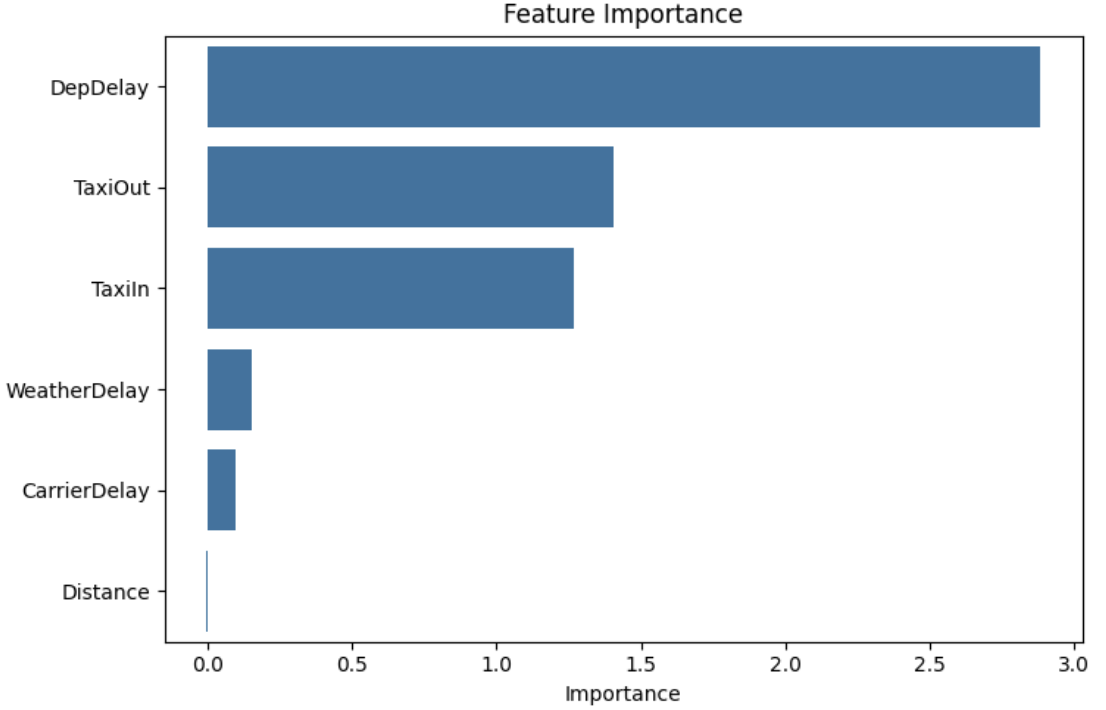
\includegraphics[width=\textwidth]{../img/diag.png} % Replace with your image path
      \caption{Feature importance analysis showing the impact of each predictor on flight delays.}
      \label{fig:feature_importance}
    \end{minipage}
    \hfill % Adds horizontal space between figures
    \begin{minipage}[b]{0.48\textwidth}
      \centering
      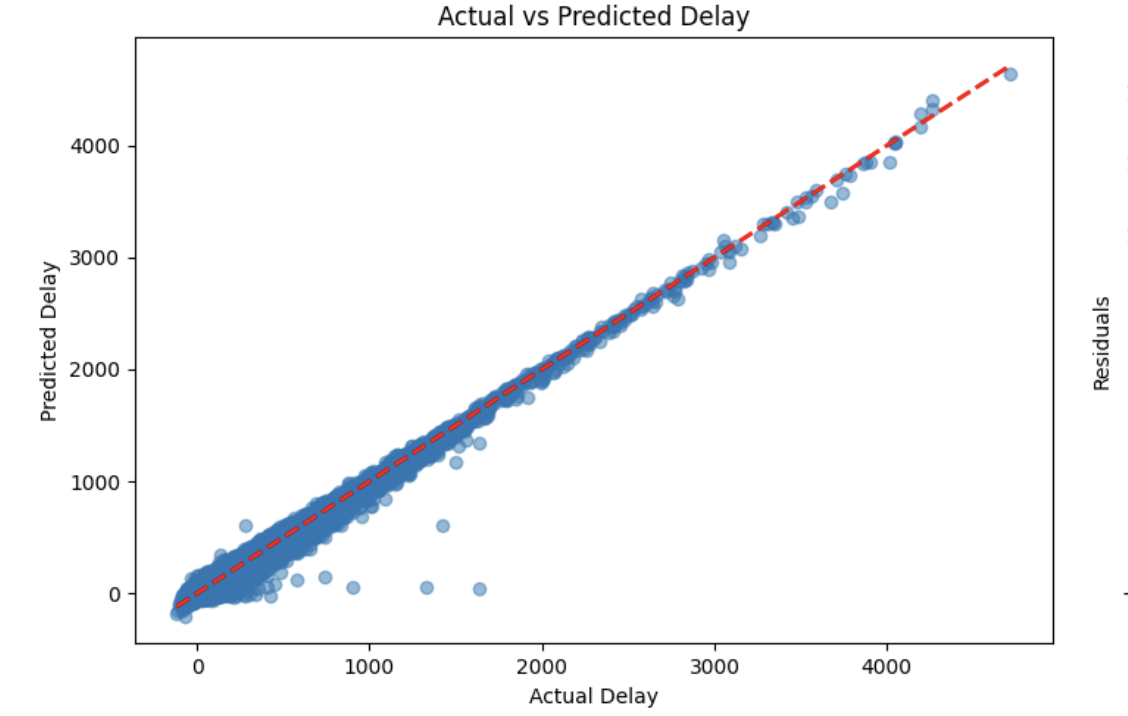
\includegraphics[width=\textwidth]{../img/avsp.png}
      \caption{Actual vs Predicted Delay showing the model’s prediction accuracy.}
      \label{fig:actual_vs_predicted}
    \end{minipage}
  \end{figure}


